\documentclass{beamer}

\usepackage[slovene]{babel}
\usepackage{amsfonts,amssymb}
\usepackage{amsmath}
\usepackage[utf8]{inputenc}
\usepackage{lmodern}
\usepackage[T1]{fontenc}
\usepackage{mathtools}
\usepackage{graphicx}

\graphicspath{{images/}}



\usetheme{Warsaw}

\newcommand{\norm}[1]{\left\lVert#1\right\rVert}

\def\qed{$\hfill\Box$} 
\newtheorem{izrek}{Izrek}
\newtheorem{trditev}{Trditev}
\newtheorem{posledica}{Posledica}
\newtheorem{lema}{Lema}
\newtheorem{definicija}{Definicija}
\newtheorem{opomba}{Opomba}
\newtheorem{primer}{Primer}
\newtheorem{zgled}{Zgled}
\newtheorem{zgledi}{Zgledi uporabe}
\newtheorem{zglediaf}{Zgledi aritmetičnih funkcij}
\newtheorem{oznaka}{Oznaka}
\newtheorem{dokaz}{Dokaz}

\newtheorem{dokaz2}{Dokaz}
\newtheorem{proof1}{Interactive proof for GNI with private coins }
\newtheorem{claim}{Claim}


\title{Najkrajša pot z odstranljivimi ovirami}
\author{ Gašper Terglav} 
\institute[FMF] % (optional)

\begin{document}

\begin{frame}
    \titlepage
\end{frame}


\begin{frame}
    \frametitle{Primer problema}

    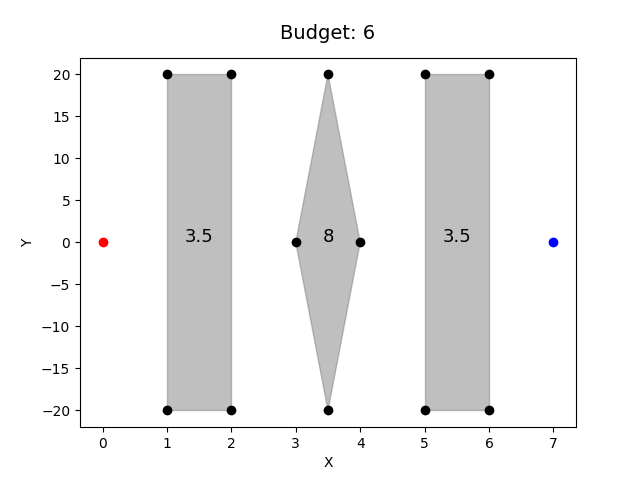
\includegraphics[width=1\textwidth]{err1.png}

\end{frame}

\begin{frame}
    \frametitle{Viability graf}

    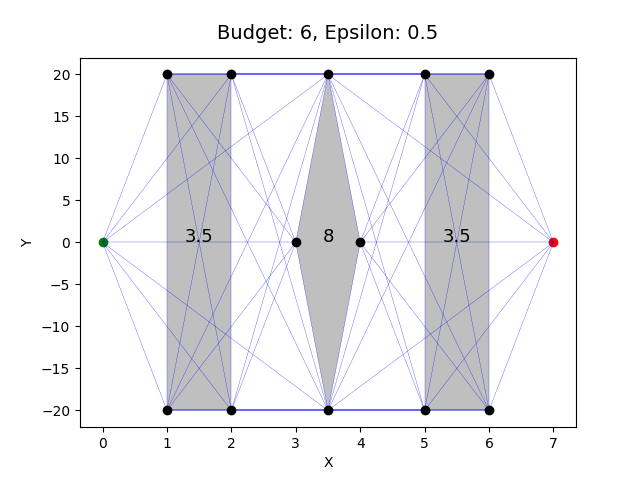
\includegraphics[width=1\textwidth]{errGraph1.png}

\end{frame}

\begin{frame}
    \frametitle{Rešitev}
    Izberemo parameter natančnosti $\epsilon$.
    Če ima viabilty graf vozlišča $v \in V$, potem ima nov graf vozlišča oblike $v_i \in V$, kjer $i = 0, \epsilon, 2\epsilon, \dots, \lceil budget/\epsilon\rceil$.
    \pause
    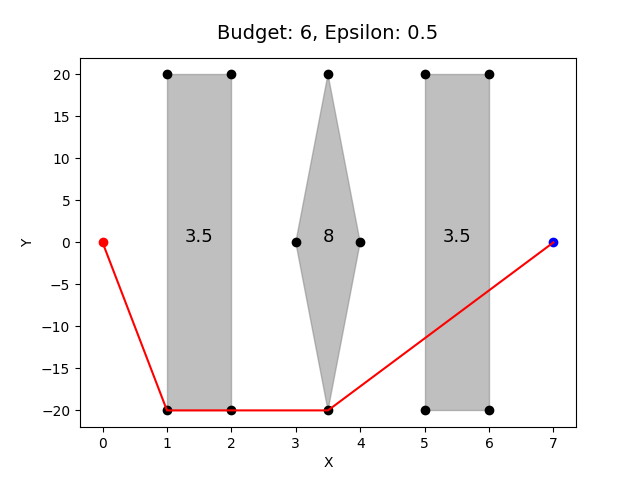
\includegraphics[width=0.8\textwidth]{errPath1.png}

\end{frame}

\begin{frame}
    \frametitle{Rešitev}
    Napaka algoritma je $1+2\epsilon$ v ceni.

    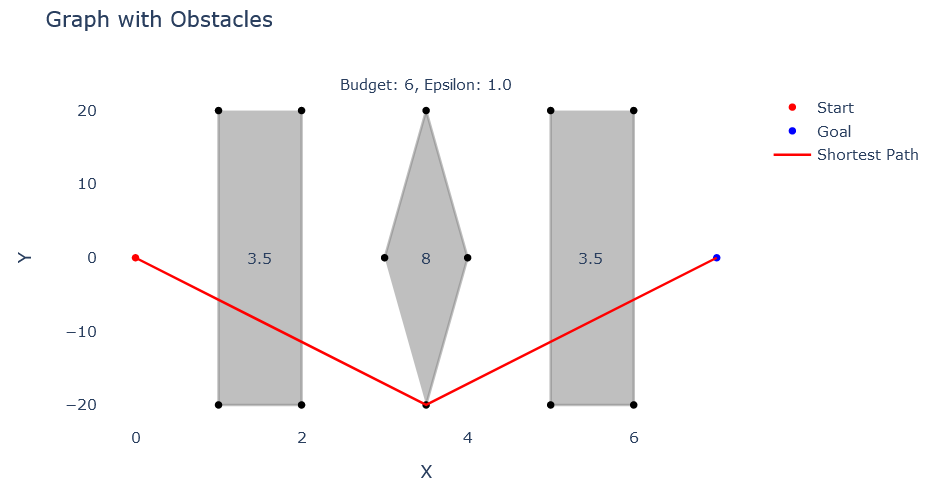
\includegraphics[width=1\textwidth]{errorProblem1.png}

\end{frame}


\begin{frame}
    \frametitle{Naivni algoritem}
    Za vsak par točk $v,u$ in vsak rob ovire $e$, pogledam,če $\overline{vu}$ seka $e$. Če ja, dodam ceno ovire $e$ k ceni $\overline{vu}$. V graf dodam vse daljice s ceno manj od budgeta.
    \pause
    Časovna zahtevnost $O(n^3)$. Zahtevnost celotnega algoritma je potem  $O(n^3/\epsilon)$
    \pause
    \begin{table}[h]
        \centering
        \begin{tabular}{|c|c|c|c|c|}
            \hline
            & \multicolumn{4}{c|}{n (število oglišč)} \\
            \cline{2-5}
            & 40 & 180 & 360 & 860 \\
            \hline
            Čas & 0.5s & 36s &  301s &  1ura 16min\\
            \hline
        \end{tabular}
        \caption{Vpliv $n$ na čas iskanja poti}
        \label{tab:1}
    \end{table}

\end{frame}

\begin{frame}
    \frametitle{Naivni algoritem}
   
    \begin{table}[h]
        \centering
        \begin{tabular}{|c|c|c|c|c|}
            \hline
            & \multicolumn{4}{c|}{$\epsilon$} \\
            \cline{2-5}
            & 0.01 & $10^{-3}$ & $10^{-4}$ & $10^{-5}$ \\
            \hline
            Čas & 0.5s & 5s &  57s & memory full \\
            \hline
           
        \end{tabular}
        \caption{Vpliv vrednosti $\epsilon$ na čas iskanja poti}
        \label{tab:2}
    \end{table}


\end{frame}

\begin{frame}
    \frametitle{Naivni algoritem}
    Problem:

    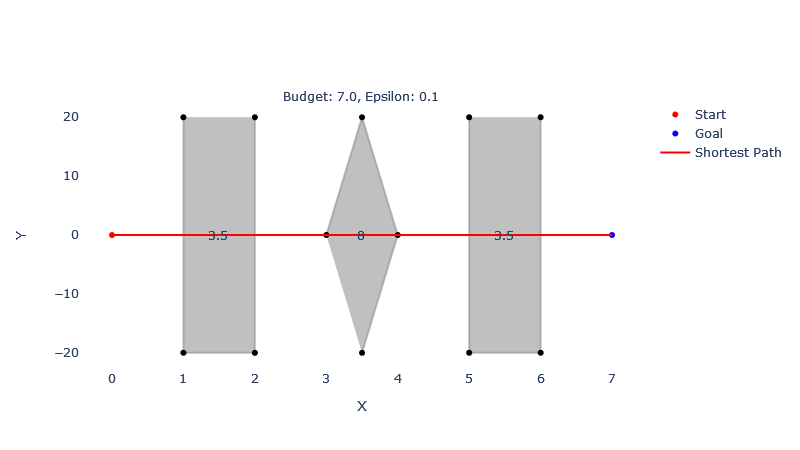
\includegraphics[width=1\textwidth]{naiveErr.png}
\end{frame}

\begin{frame}
    \frametitle{Sweep algoritem}
    
    Za vsako točko $v$, ostale točke uredim glede na kot z vodoravno premico in jih nato pregledam po vrsti. Robove ovir shranjujem v AVL drevo.

    \pause

    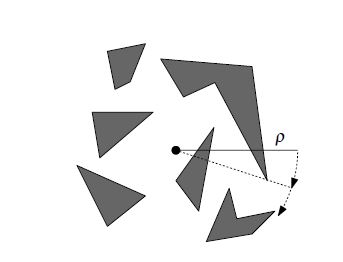
\includegraphics[width=0.4\textwidth]{sweep.png}

    \pause

    Časovna zahtevnost $O(n^3)$. Zahtevnost celotnega algoritma je potem  $O(n^3/\epsilon)$

    
\end{frame}

\begin{frame}
    \frametitle{Sweep algoritem}
    \begin{table}[h]
        \centering
        \begin{tabular}{|c|c|c|c|c|}
            \hline
            & \multicolumn{4}{c|}{n (število oglišč)} \\
            \cline{2-5}
            & 40 & 180 & 360 & 860 \\
            \hline
            Čas & 0.7s & 50s &  393s &  1ura 28min\\
            \hline
        \end{tabular}
        \caption{Vpliv $n$ na čas iskanja poti}

    \end{table}
   
    \begin{table}[h]
        \centering
        \begin{tabular}{|c|c|c|c|c|}
            \hline
            & \multicolumn{4}{c|}{$\epsilon$} \\
            \cline{2-5}
            & 0.01 & $10^{-3}$ & $10^{-4}$ & $10^{-5}$ \\
            \hline
            Čas & 1s & 11s & 126s  &  memory full \\
            \hline
           
        \end{tabular}
        \caption{Vpliv vrednosti $\epsilon$ na čas iskanja poti}
    \end{table}
\end{frame}

\begin{frame}
    \frametitle{Sparse algoritem}
    
    \begin{itemize}

        \item Določimo navpično premico $p$, ki razdeli točke na dva množici približno enake moči.
        Za vsako točko $v$ je $v'$ njena projekcija na $p$. 
        \pause

        \item  Poiščemo prvi rob ovire z navpičnim naklonom, ki seka $\overline{vv'}$. Označimo presečišče z $x$. Če obstaja presečišče roba s $p$ (označimo ga z $y$). Dodamo v graf $\overline{xy}$.
        \pause
        \item  Ponovimo za prvi negativen rob.
        \pause
        \item  Rekurzivno ponovimo na levi in desni strani $p$.
        \pause
        \item Ponovimo vse do sedaj $\lceil 1/\epsilon\rceil$-krat, le da vsakič zarotiramo ravnino za kot $2\pi \epsilon$. 
    \end{itemize} 

\end{frame}

\begin{frame}
    \frametitle{Sparse algoritem}
    
    Primer:

    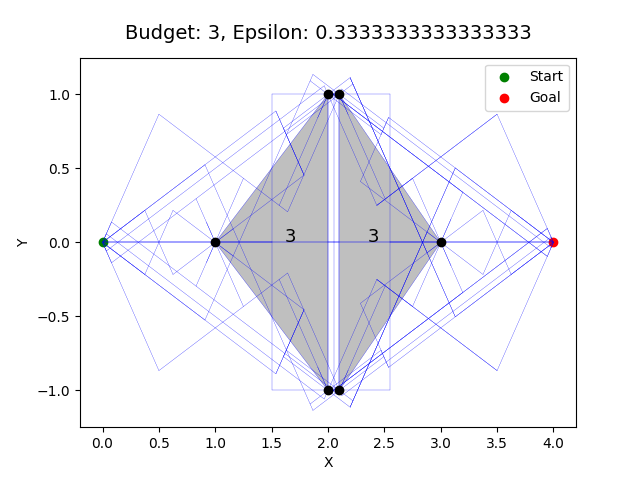
\includegraphics[width=1\textwidth]{sparseGraph.png}

\end{frame}

\begin{frame}
    \frametitle{Sparse algoritem}

    Za algoritem je treba določiti samo cene navpičnih in vodoravnih poti. Rešitev: persistent search tree.

    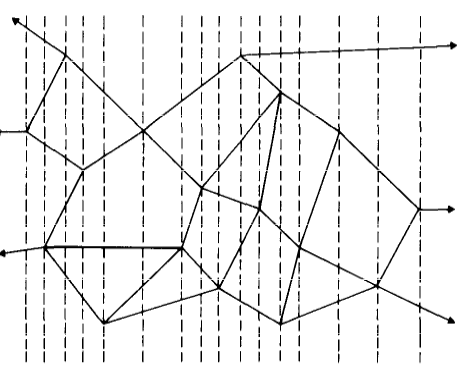
\includegraphics[width=0.7\textwidth]{slabs.png}
    
\end{frame}

\begin{frame}
    \frametitle{Sparse algoritem}

    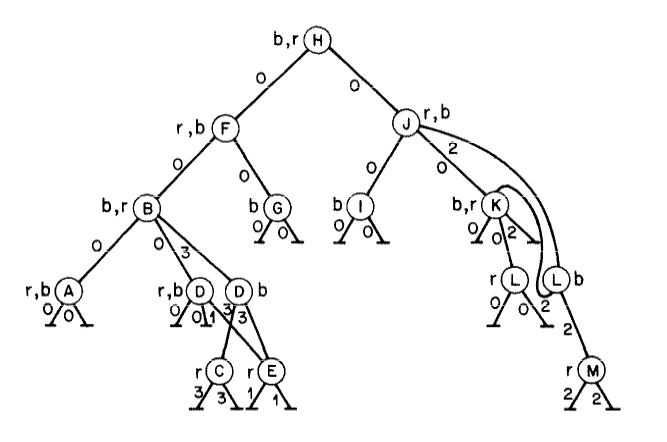
\includegraphics[width=1\textwidth]{psTree.png}

\end{frame}


\begin{frame}
    \frametitle{Sparse algoritem}

    Časpvna zahtevnost bi morala biti $O(\frac{nh}{\epsilon^2} \log n \log \frac{n}{\epsilon})$.

    \begin{table}[h]
        \centering
        \begin{tabular}{|c|c|c|c|c|c|}
            \hline
            & \multicolumn{5}{c|}{$\epsilon$} \\
            \cline{2-6}
            & 0.5 & 0.25 & 0.1 & 0.01 & 0.001 \\
            \hline
            Čas & 0.01s & 0.03s & 0.5s & 31s & 4651 \\
            \hline
        \end{tabular}
        \caption{Vpliv vrednosti $\epsilon$ na čas iskanja poti}
    \end{table}

    \begin{table}[h]
        \centering
        \begin{tabular}{|c|c|c|c|}
            \hline
            & \multicolumn{3}{c|}{n} \\
            \cline{2-4}
            & 15 & 40 & 180 \\
            \hline
            Čas & 0.37s & 24s &  905s \\
            \hline
        \end{tabular}
        \caption{Vpliv $n$ na čas iskanja poti ($\epsilon$ = 0.2)}

    \end{table}

\end{frame}

\end{document}